\documentclass[12pt,addpoints]{exam}
\usepackage{amsmath,amssymb} % standard math extensions
\usepackage{tikz} % for graphs and figures
\usepackage{pgfplots}
\usetikzlibrary{patterns}
\usepackage{graphicx} % for including the JAC logo
\usepackage{version} % for including and excluding various elements easily
\usepackage{xcolor} % for changing text colour; only used while working on the draft.  Sample use: {\color{red} This text will appear in red.}
\usepackage{nicefrac} % for nice slanted fractions
\usepackage{bm} % so I can use a bold font in math mode with \bm{stuff}
\usepackage{enumitem}
\usepackage{comment}

\newcommand\mystrut{\rule{0pt}{\ht\strutbox}} % just to adjust the location of the rational exponent on e in the curve sketching question; from https://tex.stackexchange.com/questions/603294/how-do-i-raise-the-vertical-height-of-an-exponent-in-a-math-equation-even-higher

%%%%%%%%%%%%%%%%%%%%
% Extra inverse trig operators in case they're needed:

\DeclareMathOperator{\arcsec}{arcsec}
\DeclareMathOperator{\arccot}{arccot}
\DeclareMathOperator{\arccsc}{arccsc}


% Version selections! %%%%%%%%%%%%%%%%%%%%%%%%%%%

%\includeversion{coverpage}
\excludeversion{coverpage}

%\includeversion{spacing}
\excludeversion{spacing}

\includeversion{answers}
%\excludeversion{answers}


%%%%%%%%%%%%%%%%%%%%%%%%%%%%%%%%%%%%%
% EXAM COURSE, TIME, DATE, INSTRUCTIONS INFO
%%%%%%%%%%%%%%%%%%%%%%%%%%%%%%%%%%%%%

% change the following five definitions as needed
\newcommand{\Date}{December 2025}
\newcommand{\Time}{{\upshape 14h--17h}}
\newcommand{\Course}{Differential Calculus}
\newcommand{\CourseNumber}{201-DDD-05}
\newcommand{\Instructors}{Mohammad Bardestani, Olivier Dubois, Gustavo Felisberto Valente, Kenzy Malek, Luiz Kazuo Takei}  % Quick-and-dirty trick to prevent hyphenation of a name, if needed; use \mbox, for example: Ivo \mbox{Pendev}
%
%
%% FAKE DATA  to help with exam security during test creation; comment out before printing final draft!
%\renewcommand{\CourseNumber}{201-AS1-RE}
%\renewcommand{\Course}{Algebra}
%\renewcommand{\Date}{16 May 2011}

%%%%%%%%%%%%%%%%%%%%%%%%%%%%%%%%%%%%%

% How do we want the points to appear?

\pointsinmargin
\bracketedpoints

%%%%%%%%%%%%%%%%%%%%%%%%%%%%%%%%%%%%%

% exam document class formatting commands
\extrawidth{1in}
\extraheadheight{-0.25in}
\extrafootheight{-0.375in}
\renewcommand{\questionlabel}{\bfseries\thequestion.} % bold question numbers
\pagestyle{headandfoot}
\lhead{Final Examination}
\chead{\CourseNumber}
\rhead{\Date}
\headrule 
\lfoot{\iflastpage{Total: \numpoints~points}{}}
\cfoot{Page \thepage\ of \numpages}
\rfoot{\iflastpage{This is the end of the examination.}{%
		\ifincomplete{%
			Question~{\IncompleteQuestion} continues on the next page.}{%
			Please go on to the next page.}}}

% install fonts for the title page
\usepackage{oldgerm}
\newfont{\yinit}{yinit at 30pt} % changing the ##pt changes the size of the fancy D and M in Department of Mathematics
\def\yinitial#1{
\hskip-2mm
\lower2mm
\hbox{\yinit #1}
\hskip-2mm}

%%%%%%%%%%%%%%%%%%%%%%%%%%%%%%%%%%%%

%%%%%%%%%%%%%%%%%%%%%%%%
% This bit sets up the answers to be printed at the end
% Template based on http://tex.stackexchange.com/questions/15350/showing-solutions-of-the-questions-separately

\newbox\allanswers
\setbox\allanswers=\vbox{}

\newenvironment{answer}
{%
  \global\setbox\allanswers=\vbox\bgroup
  \unvbox\allanswers
}%
{%
  \bigbreak
  \egroup
}

\newcommand{\showallanswers}{\par\unvbox\allanswers}
%
%%%%%%%%%%%%%%%%%%%%%%%%%

\let\leq\leqslant \let\geq\geqslant

\begin{document}

\begin{coverpage} % this is for the version, to include or exclude the cover page (see headmatter)
\begin{coverpages} % this affects the formatting of the cover page

\begin{center}
\vspace*{-10ex} % -8ex if we're not using that big box at the bottom for the signature
\includegraphics[scale=0.25]{jaclogovertical.jpg}
\vskip 2ex \par % 5ex if we're not using that big box at the bottom for the signature
\scshape
{\huge%
\yinitial{D}epartment of%
\hskip .6em\yinitial{M}athematics \\[.67ex]
Final Examination}
\vskip 2ex \par
{\Large\upshape\Date\\[.67ex]\Time}
\vskip 1ex \par
{\huge \Course \vskip 1ex
\CourseNumber}
\vskip 2ex % usually 5ex but with so many instructors I needed to tighten things up
\begin{minipage}[t]{6in}
\normalsize Instructors:\enspace
\hangindent = 1em
{\upshape \raggedright\Instructors}
\end{minipage}
\vskip 6ex % usually 6ex but with so many instructors I needed to tighten things up
\begin{minipage}[t]{5in}
\normalsize \hbox to \textwidth
{Student name:\enspace\hrulefill}
\vskip 2ex
\hbox to \textwidth
{Student number:\enspace\hrulefill}
\vskip 2ex
\hbox to \textwidth
%{Row and seat number:\enspace\hrulefill}
%\vskip 2ex
%\hbox to \textwidth
{Instructor:\enspace\hrulefill}
\vskip 2ex
\end{minipage}
\vskip 3ex   % usually 6ex but with so many instructors I needed to tighten things up
Instructions
\vskip 2ex
\begin{minipage}[t]{6.25in}
\begin{enumerate}\upshape
\item
Do not open this booklet before the examination begins.
\item Do not write on this cover page, except to fill in your identifying information.
\item
Check that this booklet contains
{\numpages} \if\numpages1{page}\else{pages}\fi,
excluding this cover page.
\item Write all of your solutions in this booklet and show all supporting work.
\item All of your answers should be fully simplified. 
%\item If the space provided is not sufficient, continue the solution on the opposite page.
\item An extra blank page is provided at the end of the exam in case you need more space for any solution.  If you use this page, make a note telling your teacher to look there.
%\item The only calculators allowed on this exam are models beginning with Sharp EL-531.
\item Please double check that you have no cell phone or other prohibited device on your person. (If you do have such a device present it to a teacher.)
 
\end{enumerate}
\end{minipage}
\end{center}

\vskip 1ex

\begin{center}
\large\sffamily
Calculators are not permitted for this exam.
\end{center}

%\vskip -4ex
%\nopagebreak
%
%\begin{center}
%\noindent\fbox{%
%  \parbox{\textwidth}{%
%%\large\sffamily
%%\vskip 0.8ex
%I hereby certify that I am not in possession of any unauthorized material, such as a calculator, a cell phone, a smart watch, written material, or other prohibited objects.  
%\vskip 1ex
%\hspace{8cm}  Signature:  \ \ \underline{\makebox[3.0in][l]{}}\ \
%%\vskip 0.8ex
%  }%
%}
%\end{center}


\vfill

\end{coverpages}
\end{coverpage}


%%%%%%%%%%%%%%%%%%%%%%%%%%%%%%%%%%%%%%%%%%%%%%%%%%%%%%%%%%%%%%%%%
%%%%%%%%%%%%%%%%%%%%%%%%%%%%%%%%%%%%%%%%%%%%%%%%%%%%%%%%%%%%%%%%%
%
%  AND NOW WE'RE DONE WITH THE SETUP AND WE GET TO THE ACTUAL QUESTIONS!!!
%
%%%%%%%%%%%%%%%%%%%%%%%%%%%%%%%%%%%%%%%%%%%%%%%%%%%%%%%%%%%%%%%%%
%%%%%%%%%%%%%%%%%%%%%%%%%%%%%%%%%%%%%%%%%%%%%%%%%%%%%%%%%%%%%%%%%

\begin{questions}

\setlength{\itemsep}{0.5cm}


\question[15] Evaluate the following limits, if they exist. If a limit doesn't exist, write $\infty, -\infty$ or $DNE$ as appropriate. Justify with appropriate calculations.

\begin{parts}
\part $\lim\limits_{x \to -3}\dfrac{x + \sqrt{6 - x}}{x + 3}$

\part $\lim\limits_{x \to 2^-} \dfrac{3}{x^2 - x - 2}$

\part $\lim\limits_{x \to 0}\dfrac{\tan^2 (x)}{x \sin (x)}$

\part $\lim\limits_{x \to -\infty} \dfrac{7x^3 + \sqrt{x^6 + 1}}{(3x^2 - x)(1 + 2x)}$

\part $\lim\limits_{x \to \infty} \dfrac{2\cos(3x)}{1 + 5x}$ \hfill (Hint: you may use the squeeze theorem.)
\end{parts}

\begin{answer}
	\thequestion.  (a) $5/6$  \quad (b) $-\infty$  \quad (c) $1$ \quad (d) $1$ \quad (e) $0$
\end{answer}


\question[5] Find and classify (as removable, jump or infinite) all discontinuities of 
\[
f(x) =
\begin{cases}
\dfrac {5x^2 + 4x - 1} {x - 3} & \text{if \( x \leq 1 \) and } \\[1.5ex]
\dfrac {x^2 - 9} {x^2 - 5x + 6} & \text{if \( x > 1 \).}
\end{cases}
\]

\begin{answer}
	\thequestion.  infinite discontinuity at $x=2$ and removable discontinuity at $x=3$
\end{answer}

\question[5] Use the limit definition of the derivative to find $f'(x)$ where ${\displaystyle f(x) = \frac{5}{x^2-2}}$.

\begin{answer}
	\thequestion.  $\frac{-10x}{(x^2-2)^2}$
\end{answer}


\question[13] Find $\displaystyle \frac{dy}{dx}$ for each of the following. \textbf{Do not simplify your answers.}

\begin{parts}
	\part $y=\dfrac{5}{x}+\pi^e+\log_3 (x) +\arcsin(x)$
	\part $y=\dfrac{7+e^x}{\tan^3 (x)}$
	\part $y = \cos^2\Big( (3x^2 + 1)^4 \Big)$
	\part $y = 5(2x+3)^{2-x}$
\end{parts}

\begin{answer}
\thequestion.  (a) $\frac{-5}{x^2} + \frac{1}{x \ln 3} + \frac{1}{\sqrt{1-x^2}}$  \quad (b) $\frac{e^x \tan^3 (x) - 3(7 + e^x) \tan^2(x) \sec^2(x)}{\tan^6(x)}$  \quad (c) $-48 \cos((3x^2+1)^4) \sin((3x^2+1)^4) (3x^2+1)^3 x$ \quad (d) $5(2x+3)^{2-x} \left( -\ln(2x+3) + \frac{4-2x}{2x+3} \right)$
\end{answer}

\question[4] Given the equation $e^{xy} + 3 = \dfrac{x}{\sin(y)}$, find $\dfrac{dy}{dx}$.

\begin{answer}
	\thequestion.  $\frac{\sin(y) - y \sin^2(y) e^{xy}}{x \cos(y) +  x \sin^2(y)e^{xy}}$
\end{answer}

\question[4] Consider the curve given by $y = x - \sqrt{4x-8}$. Give an equation for the tangent line at $x=6$.

\begin{answer}
	\thequestion.  $y = \frac{x}{2} - 1$
\end{answer}

\question[6] An inverted cone that is 20 cm tall with a radius of 8 cm is initially full of water. The water drains at a constant rate of 15 cm$^3$ per second. We want to find the rate at which the water level is falling when the water is halfway down the cone. (The volume of a cone is given by $V = \frac{1}{3} \pi h r^2$.)
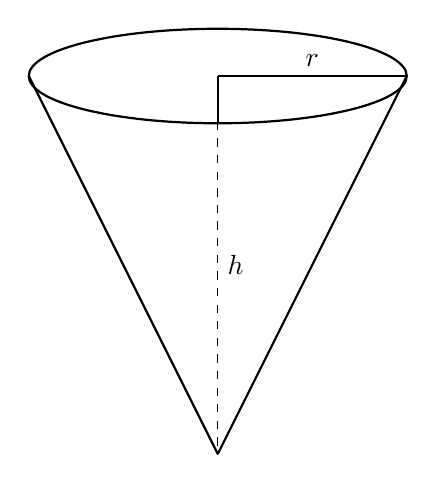
\begin{tikzpicture}[scale=1.2]

  % Base ellipse (top of inverted cone)
  \draw[thick] (-2,0) arc[start angle=180,end angle=360,x radius=2cm, y radius=0.5cm];
  \draw[thick] (2,0) arc[start angle=0,end angle=180,x radius=2cm, y radius=0.5cm];

  % Cone sides
  \draw[thick] (-2,0) -- (0,-4);
  \draw[thick] (2,0) -- (0,-4);

  % Height
  \draw[thick] (0,0) -- (0,-0.485);
  \draw[dashed] (0,-0.485) -- (0,-4);
  \node[right] at (0,-2) {\( h \)};

  % Radius
  \draw[thick] (0,0) -- (2,0);
  \node[above] at (1,0) {\( r \)};

\end{tikzpicture}

\begin{answer}
\thequestion.  $\frac{15}{16\pi}$ cm/s
\end{answer}



\question[12] Given
\[
	f(x) = \dfrac{-4(x+1)(x+4)}{(x-2)^2} \quad , \quad f'(x) = \dfrac{36(x+2)}{(x-2)^3} \quad , \quad f''(x) = \dfrac{-72(x+4)}{(x-2)^4},
\]
sketch the graph of $f(x)$ and clearly list
\begin{enumerate}[label=(\roman*)]
	\item domain of $f(x)$
	\item $x$-intercepts and $y$-intercept of $f$
	\item vertical and horizontal asymptotes of $f$
	\item relative (local) extrema of $f$
	\item point(s) of inflection of $f$
	\item intervals where $f$ is increasing, decreasing, concave upward, concave downward.
\end{enumerate}

\begin{answer}
	\thequestion.  (i) domain $ = \mathbb{R} \backslash \{2\}$ \quad (ii) $x$-intercepts: $(-1,0)$ and $(-4,0)$, $y$-intercept: $(0,-4)$ \quad (iii) v.a.: $x=2$, h.a.: $y = -4$ \quad (iv) local max. at $x=-2$, no local min. (increasing on $(-\infty, -2)$ and $(2, \infty)$, decreasing on $(-2, 2)$) \quad (v) point of inflection at $x=-4$ (concave up on $(-\infty, -4)$, concave down on $(-4,2)$ and $(2,\infty)$)
	
	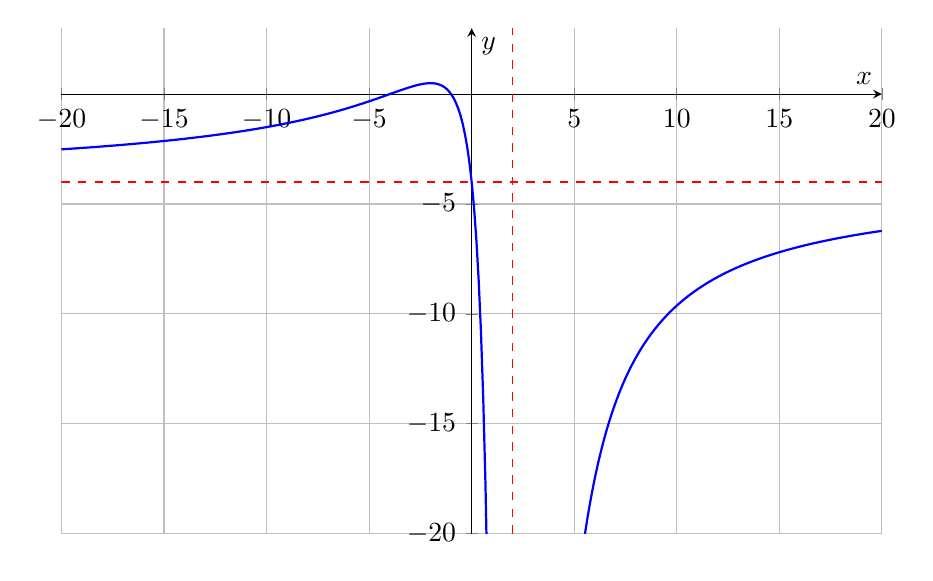
\begin{tikzpicture}
		\begin{axis}[
			axis lines = middle,
			xlabel = $x$,
			ylabel = {$y$},
			xmin=-20, xmax=20,
			ymin=-20, ymax=3,       % zoom in to see features
			grid=both,
			width=12cm, height=8cm,
			samples=200,
			restrict y to domain=-25:3,
			]
			% Left of the vertical asymptote
			\addplot[blue, thick, domain=-20:1.9999] 
			{-4*(x+1)*(x+4)/((x-2)^2)};
			
			% Right of the vertical asymptote
			\addplot[blue, thick, domain=2.01:20] 
			{-4*(x+1)*(x+4)/((x-2)^2)};
			
			% Vertical asymptote at x=2
			\addplot[dashed, red] coordinates {(2,-20) (2,3)};
			
			% Horizontal asymptote at y=-4
			\addplot[dashed, red] coordinates {(-20,-4) (20,-4)};
			
			% Mark zeros
			%\addplot[mark=*, only marks, blue] coordinates {(-4,0) (-1,0)};
		\end{axis}
	\end{tikzpicture}
\end{answer}


\question[6] A cylindrical can is constructed from a rectangular sheet of metal (for its side wall) and two circles that have been cut from square pieces (for its top and bottom.)

If the can's volume must be 1000 cm${}^3$, find the dimensions of the can that will minimize the total amount of starting material (the rectangle and both squares).

The volume of a cylinder is given by $V = \pi r^2 h$.

\vspace{1cm}

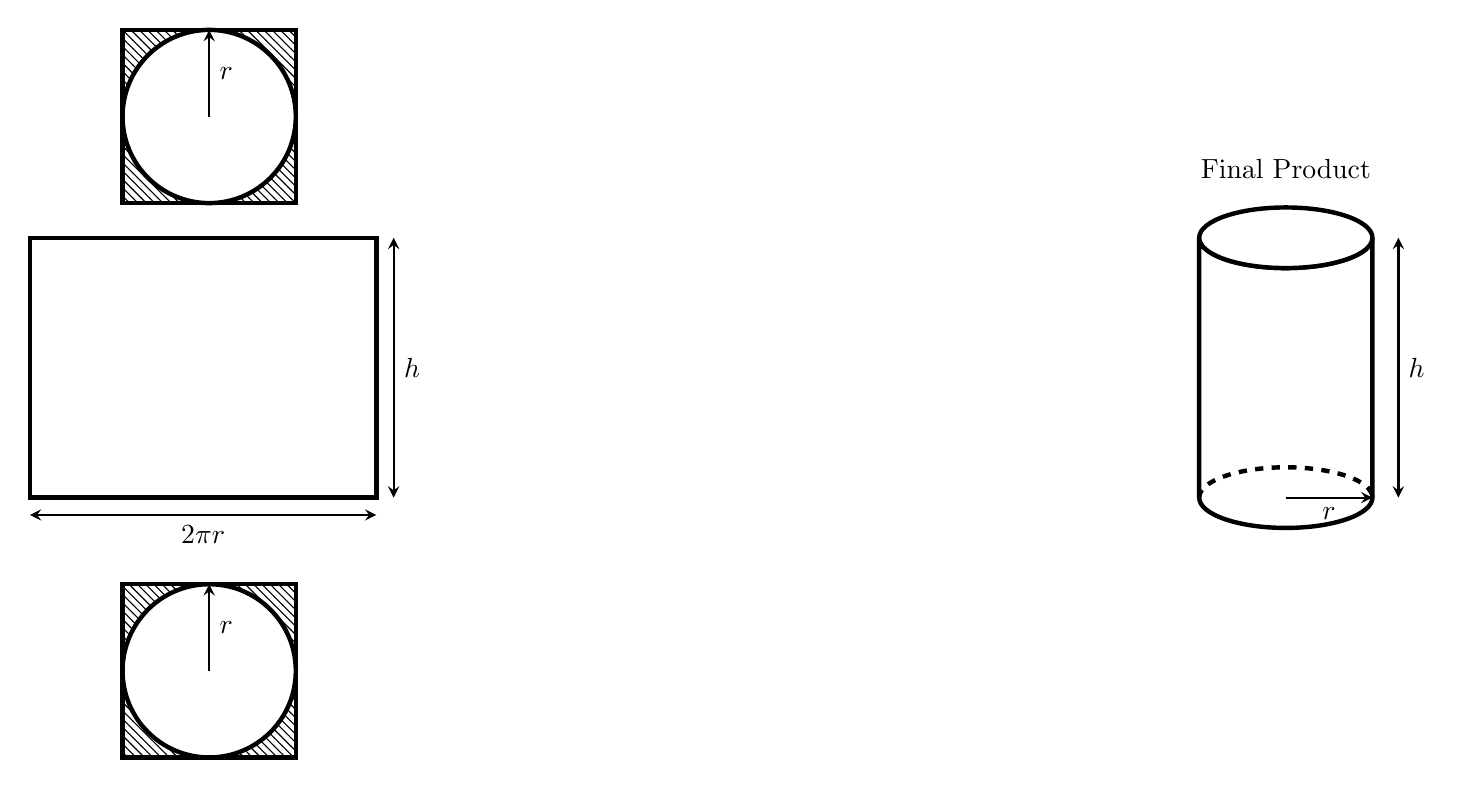
\begin{tikzpicture}[scale=1.1]
    % Define parameters
    %\def\sqshift{1.5}
    \def\sqshift{1.07}
    \def\height{3}
    \def\pistonheight{2}
		\def\pistonthickness{0.3}
    \def\tuberadius{0.15}
    \def\tubeheight{4}
% Square for top
\begin{scope}[shift={(\sqshift,0)}]
    \draw[ultra thick] (0,0) rectangle (2,2);
    \fill[pattern=north west lines] (0,0) rectangle (2,2);
    \draw[ultra thick,fill=white] (1,1) circle (1);
    \draw[ultra thick] (0,0) rectangle (2,2);
    
    \draw[->,>=stealth,thick] (1,1) -- (1,2) node[midway,right] {$r$};
    %\draw[<->,>=stealth,thick] (0,-0.3) -- (2,-0.3) node[midway,below] {$2r$};
\end{scope}

% Square for bottom  
\begin{scope}[shift={(\sqshift,-6.4)}]
    \draw[ultra thick] (0,0) rectangle (2,2);
    \fill[pattern=north west lines] (0,0) rectangle (2,2);
    \draw[ultra thick,fill=white] (1,1) circle (1);
    \draw[ultra thick] (0,0) rectangle (2,2);
    
    \draw[->,>=stealth,thick] (1,1) -- (1,2) node[midway,right] {$r$};
    %\draw[<->,>=stealth,thick] (0,-0.3) -- (2,-0.3) node[midway,below] {$2r$};
\end{scope}

% Rectangle for side
\begin{scope}[shift={(0.5,-3.4)}]
    \draw[ultra thick,fill=white] (-0.5,0) rectangle (3.5,3);
    
    \draw[<->,>=stealth,thick] (3.7,0) -- (3.7,3) node[midway,right] {$h$};
		\draw[<->,>=stealth,thick] (-0.5,-0.2) -- (3.5,-0.2) node[midway,below] {$2\pi r$};
\end{scope}

% Assembled can
%\begin{scope}[shift={(8.5,-0.4)}]
\begin{scope}[shift={(14.5,-0.4)}]
		\node at (0,0.8) {Final Product};
		
    % Bottom
    \draw[ultra thick,fill=white] (0,-3) ellipse (1 and 0.35);
    
    % Side
    \draw[ultra thick,fill=white] (-1,-3) -- (-1,0) arc (180:360:1 and 0.35) -- (1,-3);
    
    % Top ellipse outline
    %\draw[ultra thick] (-1,0) arc (180:360:1 and 0.35);
    \draw[ultra thick,dashed] (-1,-3) arc (180:0:1 and 0.35);
    
    % Top circle
    \draw[ultra thick,fill=white] (0,0) ellipse (1 and 0.35);
    
    % Dimensions
    \draw[<->,>=stealth,thick] (1.3,0) -- (1.3,-3) node[midway,right] {$h$};
    \draw[->,>=stealth,thick] (0,-3) -- (1,-3) node[midway,below] {$r$};
\end{scope}

\end{tikzpicture}

\begin{answer}
\thequestion.  $r=5$, $h = 40/\pi$
\end{answer}

\question[5] Evaluate $\displaystyle{\int_{0}^{4}(x^2-4x)}\ dx$, using the definition of the integral as a limit of Riemann sums.\\

\begin{answer}
	\thequestion.  $-32/3$
\end{answer}

The following summation formulas are provided for reference. 
\[
	\sum_{i=1}^n i = \frac{n(n+1)}{2} \qquad\qquad \sum_{i=1}^n i^2 = \frac{n(n+1)(2n+1)}{6} \qquad\qquad \sum_{i=1}^n i^3 = \left(\frac{n(n+1)}{2}\right)^2
\]

\question[12] Evaluate the integrals below.
\begin{parts}
	\part $\displaystyle \int (4\sqrt{x^3} + 2 \sin (x) - e^{2025}) \, dx$
	\part $\displaystyle \int \frac{(3x-5)^2}{x} \, dx$
	\part $\displaystyle \int \bigl(\cot (x) + \csc^3 (x) \bigr) \sin (x) \, dx$
	\part $\displaystyle \int_{1/2}^{\sqrt{3}/2} \frac{6\,dx}{\sqrt{1 - x^2}}$
\end{parts}

\begin{answer}
\thequestion.  (a) $\frac{8}{5} x{5/2} - 2 \cos(x) - e^{2025}x + C$ \quad (b) $\frac{9}{2}x^2 - 30x + 25 \ln |x| + C$ \quad (c) $\sin(x) - \cot (x) + C$ \quad (d) $\pi$
\end{answer}

\question[5] Consider a particle that moves along the number line with velocity $v(t) = e^t + 6t^2$ and initial position $s(0) = 3$. Find the position function $s(t)$ of the particle.

\begin{answer}
	\thequestion.  $s(t) =  e^t + 2t^3 + 2$
\end{answer}

\question[5] Find the area of the region between the curves $y = \sin x$ and $y = \cos x$ for $0 \leq x \leq \pi$. (Hint: the two curves intersect at $x = \pi/4$.)

\begin{answer}
	\thequestion.  $2 \sqrt{2}$
\end{answer}

\question[3] Let ${\displaystyle f(x) = \int_0^x \sqrt[3]{t-8} \, dt}$. Over what interval(s) is $f(x)$ increasing?

\begin{answer}
	\thequestion.  $(8, \infty)$
\end{answer}



\end{questions}

\begin{answers} % use the Version lines in the headmatter to control whether the answers show up here or not.
	
	\newpage
	%	\bigskip
	
	\textbf{Answers:}
	
	\bigskip
	
	
	\showallanswers
\end{answers}


\end{document}